\documentclass{article}
\usepackage[utf8]{inputenc}
\usepackage{graphicx}

%%%%%%%%%%%%%%%%%%%%%%%%%%%%%%%%%%%%%%%%%%%%%
\RequirePackage[pdftex,hidelinks]{hyperref}
% For lists
\usepackage{outlines}
\usepackage[shortlabels]{enumitem}
\usepackage{tabularx}
\usepackage{xcolor}
%%%%%%%%%%%%%%%%%%%%%%%%%%%%%%%%%%%%%%%%%%%%%

\title{Evaluating the Performance of Language Models solving ENEM: A Study of BERTimbau and GPT-3 }
\author{Desnes Nunes (desnesn@usp.br) e Ricardo Primi (rprimi@mac.com)}
\date{\today}

\begin{document}

\maketitle

\begin{abstract}

This paper examines the potential of artificial intelligence, specifically Transformer models such as BERT and GPT-3, in answering the Brazilian National High School Examination (ENEM). We analyzed the data of 916 questions administered in years 2010 to 2017 from ENEM Challenge \url{https://www.ime.usp.br/~ddm/project/enem/}. A number of models were tested based on BERTimbau embeddings, finetuned, and GPT3 with few shots and "chain of thought" training regimens. Overall, we found an accuracy score of .77 and an F1 score of .77 for the GPT3 models, which represents a new state of the art for ENEM challenge.



    % The abstract is a short text to let people understand what is the document about.
    % It should give the mains highlights of the documents.
    % This document is a template to be use in the Final Project of the EA376E class.
    % The recommendation is to use LaTeX by the application Overleaf.com, but it is also
    % possible to use Google Docs or MS-Word.
\end{abstract}

\section{Introduction}

Needless to say, recent innovations presented not only on LMs applications, but also to whole field of Machine Learning (ML) have been astonishing and seem to have an  almost unlimited application scope. This of course correlates strongly to the digital aspects present of modern life; such as banking, chat bots, meal ordering, music listening, meeting people, among many other services. Many of these rely heavily on ML processing of customer's data, in order to make Artificial Inteligence (AI) models able provide automatic suggestions, take decisions and more. Furthermore, an area that started to receive some attention recently from ML applications is education; which recently saw, for instance, works aiming ML usage in classrooms \cite{kuvcak2018machine}, as well as the so called \textit{precision education} \cite{luan2021review}. 

The paper we present explores the potential of using artificial intelligence, particularly Transformer models \cite{VaswaniAttentionAllYou2017a} such as BERT  \cite{devlin2018bert} and GPT-3 \cite{https://doi.org/10.48550/arxiv.2005.14165}, two state-of-the-art language processing models to answer the Brazilian National High School Examination (ENEM). ENEM is an important Brazilian college entrance examination, which evaluates the academic performance of high school students. The problem we aim to address is whether these models, which have achieved impressive results on a variety of natural language processing tasks, can also perform well on a standardized educational exam. Our main hypothesis is that BERT and GPT-3 will be able to accurately answer a significant number of ENEM questions, demonstrating their potential to assist in the education process.

This research is relevant for several reasons. First, it provides a novel use of BERT and GPT-3 in the educational domain, highlighting their potential in guiding future developments in the use of artificial intelligence in education, such as automatic scoring of achievement tests, automatic writing feedback for assessments, and the adoption of AI-powered tools to assist educators in developing adaptive tests and adaptive learning programs. Second, the findings of this research could have significant consequences for the education sector, potentially leading to the adoption of AI-powered tools for psychometric analysis of ENEM exams, including predicting the difficulty of questions, developing new items, and ultimately assisting in the creation of adaptive ENEM tests. Third, it contributes to the growing body of research that attempts to understand the intelligence underlying the language models. Are they capable of understanding? Can they justify their answers by providing human-like explanations of their reasoning that humans consider intelligent?  
 
This paper presents a series of experiments investigating if BERT and GPT3 can answer ENEM questions. One important aspect related to GPT3 is the enhancement of few-shots prompt engineering techniques with \textit{chain of thought} \cite{DBLP:journals/corr/abs-2201-11903}. The idea is to enhance prompts that presents a series of intermediate reasoning steps allowing the model to break down a complex problem into smaller, more manageable steps, and to reason about each step individually before combining the results to arrive at a final answer.  In this way, the model can potentially grasp abstract concepts and manipulate them, as well as solve problems that require deep understanding of underlying principles.  This technique may improve large language models' ability to perform complex reasoning. Our main question is whether the use of a chain of thought in large language models enhance their ability to perform complex reasoning tasks, like answering ENEM questions, making them more effective in a variety of applications.

The proposed research aims to advance the benchmarks for automatically solving college entrance exam by exploring recent state of the art language models for enhancing the performance of AI on this task answering the call \textbf{ENEM Challenge}  \url{https://www.ime.usp.br/~ddm/project/enem/}. ENEM's purely textual multiple-choice questions pose a challenging problem, requiring advanced natural language processing skills. The problem has been examined in earlier research \cite{8575587} using static word embeddings and WordNet but with limited success attaining an accuracy of 26\% to 29\% of correct responses. This paper proposes to extend this approach by utilizing contextual embedding of BERTimbau and few-shot capabilities of GPT3. By doing so, we aim to improve the accuracy of our model and demonstrate the potential of AI to assist in the education process. The study is important in demonstrating the potential of AI to be used in educational tests, as well as to assess the accuracy and reliability of AI-based solutions. 


%This is an example of paper citation: BERT~\cite{devlin2018bert} is a transformer. T5~\cite{raffel2019exploring} also uses transformers.

\section{Methodology}

\subsection{Data set}

The \href{https://www.ime.usp.br/~ddm/project/enem/ENEMdataset.zip}{\underline{dataset}} is openly available and has been published by \cite{DBLP:journals/corr/abs-2201-11903}. The data presented in xml format is the result of the parsing of the real questions and alternatives presented on the ENEM tests from 2010 - 2017. Moreover, the authors have labeled each question with the following knowledge tags:

\vspace{-0.15cm}
\begin{itemize}%[leftmargin=*]
  \item Text Comprehension (TC)
  \vspace{-0.25cm}
  \item Encyclopedic Knowledge (EK)
  \vspace{-0.25cm}
  \item Image Comprehension (IC)
  \vspace{-0.25cm}
  \item Domain Specific Knowledge (DS)
  \vspace{-0.25cm}
  \item Mathematical Reasoning (MR)
\end{itemize}
\vspace{-0.05cm}

These tags have been extremely helpful since they inform if a question has an image or mention chemical elements that can't be treated as text. The entire dataset consists of 1754 items from the ENEM language and human sciences tests from 2010 to 2017. After eliminating questions that require understanding of images (IC), reading of symbols of chemical elements (CE) and mathematical reasoning (MR), the final database had 916 items. 

Each item is composed of a \textbf{header} where the main text of the item is presented; \textbf{statement} where the question  is asked to the students and \textbf{alternatives}, containing five options from which one correctly answer the question (statement).

For the fine tuning experiment with BERTimbau we split items randomly into a training set (733 questions) and a test set (183 questions). Three items were selected to create prompts and chain of thought reasoning expected for the solution to use in the few-shot experiments. 


\subsection{Transformer Models}
The models used on this work (BERT and GPT3) are based on the attention mechanism of the transformers architecture and can be illustrated as follows:

\begin{figure}[h!]
    \centering
    %\captionsetup{justification=centering}
    \caption{Illustration of BERT and GPU models architecture}
    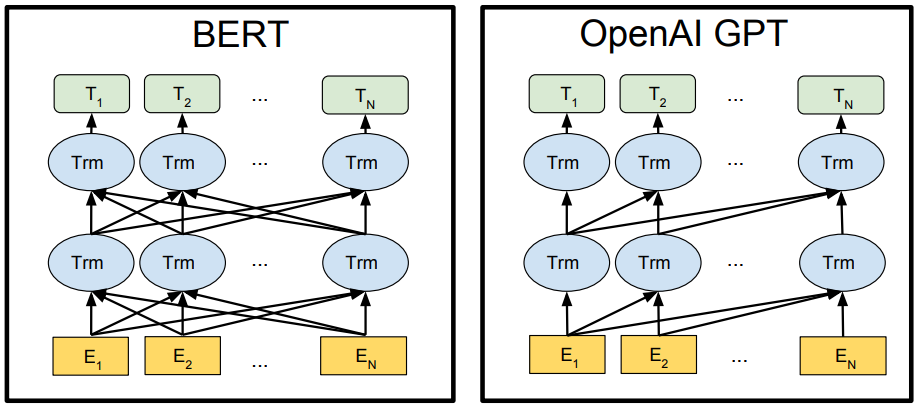
\includegraphics[width=0.75\columnwidth]{figures/4.png}
    \label{fig:3}
    \\
    \text{Source: \cite{https://doi.org/10.48550/arxiv.1907.05338}}
\end{figure}

The core mechanism of transformer's encoder and decoder is called attention.  Upon receiving tokens in continuous distributed representations (embeddings), the encoder adds a representation of the token's position within the sequence. After that, a covariance matrix is calculated between all the vectors of the tokens (illustrated as ovals in the Figure 4). This matrix stores how similar a token \textit{t} called Query is to a context called Keys (including itself). This matrix is converted into weights, called attention scores, from 0 to 1 by using the softmax function. Using these weights, a new representation of each token called Value is computed based on a weighted average of embeddings of all tokens in the sequence. Thus, if the vectors of two tokens are eventually more similar, they will be recalculated by a weighted average of both. As opposed to this, if two tokens have zero correlation, they will remain unchanged.

The transformation of the original vectors of each token enables the recreation of the vectors based on the similarity with those of the context tokens, thus enabling contextual representations. This is the core attention mechanisms.  This is explained very clearly here: \url{https://www.youtube.com/watch?v=-9vVhYEXeyQ)}. These representations are more powerful than the static word embeddings  \cite{MikolovEfficientEstimationWord2013a} used by \cite{8575587} therefore we expect better improved performance when representing ENEM questions. 

\subsection{Design and models}
We tested four models: 

\textbf{BERtimbau embeddings  \cite{souza2020bertimbau}}: We perform a forward pass for each ENEM item component (header, statement, and five alternatives), saving layer 12 embeddings  for each component. An overall embedding was created by averaging each token embedding that makes up each component. We then calculated the cosine similarity between each header/statement and alternative, and selected the one with the highest similarity as the correct alternative. In addition, we saved the embeddings of the [CLS] special tokens and selected the alternative whose embedding was most similar to the embeddings of the [CLS] question.

\textbf{BERtimbau fine tuning}: We created five examples for each item by concatenating its header, statement, and alternatives. We have specified a special [SEP] token between the header/statement and the alternative text. Therefore, in the BERT model, the first segment consists of the header/statement text and the second segment consists of the alternative text. Each example had a target label of 1 if it was paired with the correct alternative and 0 otherwise.  There are therefore five instances of headers/statements with one alternative for each. Therefore, we will have an unbalanced set of examples since only 20\% will be correct and 80\% will be incorrect. We therefore over-sampled the correct examples by repeating them four times on the training set. We started this model with pre-trained BERTimbau wheigths and trained on the test set for 3 epochs with learning rate on the test set for 3 epochs with learning rate $lr = 5e-05$.

\textbf{GPT3 with few shot}: By utilizing the few-shot learning regime of the GPT-3, an algorithm was developed to input and analyze multiple queries into the model that contained the question and its alternative answers.  We provided ENEM items as inputs for GPT3 and analyzed its results. We set up three examples as a prompt and then presented an item with it's five alternatives. The model was found to perform better when it received five inputs per question, for example, five queries containing the question, all alternatives, and which alternative was correct. Token generation was not requested from the model. Rather, we analyze the likelihood of each token among the alternatives. By aggregating the log probabilities of each token that comprises the alternative, we calculate the probability of each alternative as follows (where \textit{a} is the alternative - 1 to 5, \textit{i} is the token and \textit{N} is the total number of tokens): 

%\vspace{-0.75cm}
\begin{equation} \label{eq1}
%\begin{split}
probability(alternative_{a}) = e^{\left(\sum_{i}^{N} logprobs[i]/N\right)}
%\end{split}
\end{equation}
We used the following parameters on the GPT3 API: item temperature = 0, max\_tokens = 1, top\_p = 1, frequency\_penalty=0, presence\_penalty=0, echo=True and logprobs=5.


\textbf{GPT3 with chain of thought}: In this model, the only difference from the previous one is that the prompt contained an explanation of why the correct alternative was selected. After that, we asked for the generation of the correct alternative and explanations. 

The global performance of the model was evaluated using the global accuracy score and the F1 score by combining \textbf{precision}  (the proportion of true correct alternatives out of true positives plus false positives) and  \textbf{recall}  (the true correct alternatives out of those classified as correct by the model) into one metric by taking their harmonic mean. We expect to achieve global accuracy above 29\%, which was the baseline reported in \cite{8575587}.

% \begin{figure}[h!]
%     \centering
%     \captionsetup{justification=centering}
%         \caption{Illustration of a N-BERT model and its sesame street mascot}
%     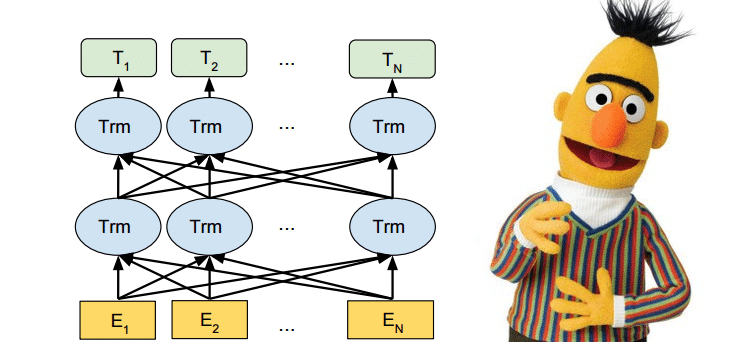
\includegraphics[width=1.0\columnwidth]{Images/3.png}
%     \label{fig:3}
%     \\
%     \text{\footnotesize Source:\cite{morris2019}}
% \end{figure}

% \begin{figure}[ht]
% \centering
% 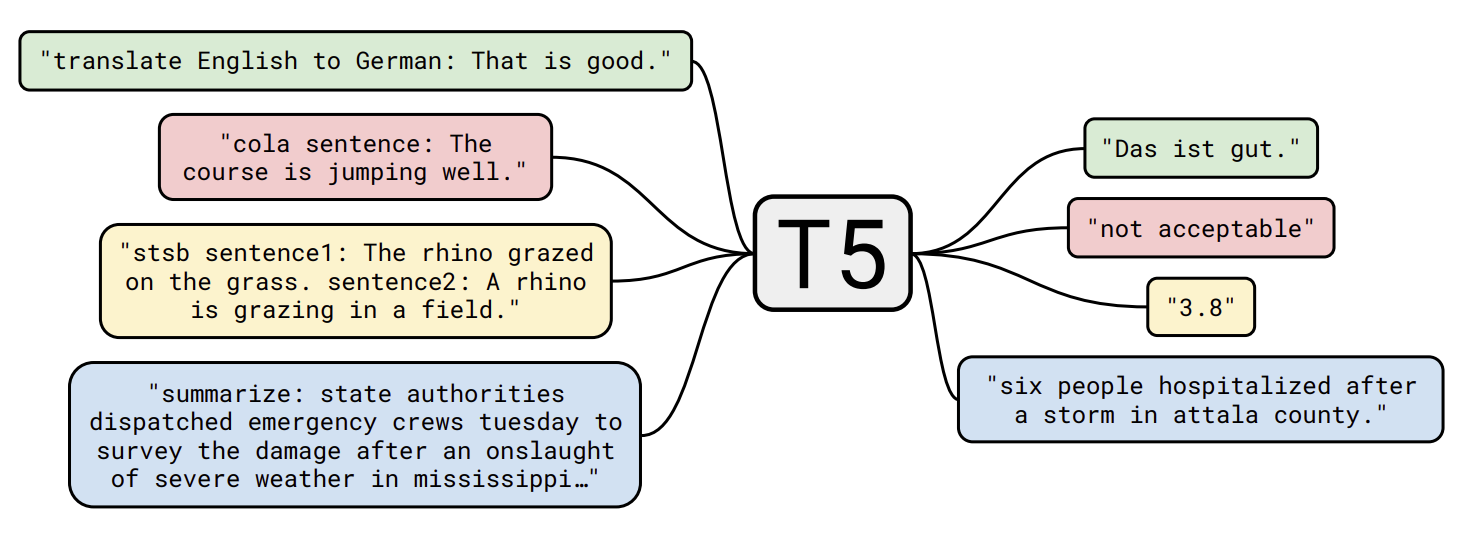
\includegraphics[width=.77\textwidth]{figures/t5.png}
% \caption{\label{fig:t5}Figure example.}
% \end{figure}

% Figure~\ref{fig:t5} is an example of figure citation.
%{\color{red}TODO: Describe XML}

\section{Experiments}

The experiments using the methodology described above were developed in python and R language. Code and data are available in github repository \url{https://github.com/rprimi/enem_challenge}. Table 1 present the main results of our evaluation of the experiments.

%\vspace{-0.05cm}
%\begin{itemize}%[leftmargin=*]
%  \item temperature = 0
%  \vspace{-0.25cm}
%  \item max\_tokens = 1
%  \vspace{-0.25cm}
%  \item top\_p = 1
%  \vspace{-0.25cm}
%  \item frequency\_penalty=0
%  \vspace{-0.25cm}
%  \item presence\_penalty=0
%  \vspace{-0.25cm}
%  \item echo=True
%  \vspace{-0.25cm}
%  \item logprobs=5
%\end{itemize}
%\vspace{-0.05cm}

% \begin{table}[h!]
%     % \centering
%     \caption{Tabela simples}
%     \begin{tabularx}{ l l }
%     \hline
%         cell1 & cell2\\   \hline
%         cell4 & cell5\\    \hline
%         cell7 & cell8\\    \hline
%     \end{tabularx}
%     \\
%     \vspace{0.25cm}
%     \text{\footnotesize Source: Own authorship, 2022.}
%     \label{ta:tabela1}
% \end{table}


%\begin{center}
%\begin{tabular}{|| l c ||} 
% \hline
% \ \ \ \ \ \ \ \ \ \ \ \ \ \ Model & Accuracy \\ [0.5ex] 
% \hline\hline
% text-davinci-002 0-shot no CoT & 77.29\% \\ 
% \hline
% text-davinci-003 0-shot no CoT & B\% \\ 
% \hline
% text-davinci-002 few-shots no CoT & C\% \\ 
% \hline
% text-davinci-002 few-shots with CoT & D\% \\
% \hline
% text-davinci-003 few-shots no CoT & E\% \\
% \hline
% text-davinci-003 few-shots with CoT & F\% \\
% \hline
%\end{tabular}
%\end{center}

\begin{center}
\begin{tabular}{ | l | l | l | }
\hline
	\  & \  & \  \\ \hline
	\textbf{Model} & \textbf{Accuracy} & \textbf{F1} \\ \hline
	  BERTIMbau Embeddings & \  & \  \\ \hline
	     Heading & 20\% & 0.19 \\ \hline
	     Statement & 21\% & 0.21 \\ \hline
	     [CLS] & 20\% & 0.19 \\ \hline
	\  & \  & \  \\ \hline
	  BERTIMbau Finetuned & 57\% & 0.41 \\ \hline
	\  & \  & \  \\ \hline
	  GPT3 & \  & \  \\ \hline
	    Few shot  davinci-002 & 77\% & 0.77 \\ \hline
	    Few shot  davinci-003 & 77\% & 0.77 \\ \hline
	    Chain of Thought  davinci-002 & \  & \  \\ \hline
	    Chain of Thought  davinci-002 &  &  \\ \hline
\end{tabular}
\end{center}

\section{Conclusion}

%{\color{red}TODO: conclusion}

\section{Future Work}

A future work would certainly be focused on the development of questions with a certain knowledge base with the usage of LMs such as GPT-3 and T5, for instance.

% Usando a bibliografia com arquivo no formato bibtex, (ver arquivo main.bib que faz parte desse projeto)
\bibliographystyle{plain}
\bibliography{main.bib}

\end{document}
